\begin{document}
\onecolumngrid
\begin{bibunit}
\begin{center}
 {\Large\textbf{Supplementary Information}}
\end{center}
\vspace*{.5cm}
\renewcommand{\figurename}{\textbf{Fig.}}
\renewcommand{\theequation}{S\arabic{equation}}
\renewcommand{\thefigure}{S\arabic{figure}}
\setcounter{equation}{0}
\setcounter{figure}{0}
\setcounter{section}{0}
This supplement provides further details about the derivation of the models and analysis methods used for our experiment.
In Sec. I, we derive the effective Hamiltonian in both position and momentum space representations. In Sec. II, we elaborate on the geometry reconstruction. In Sec. III, we describe our simulations based on the truncated Wigner approximations and provide additional comparisons between experimental data and simulation results.

\section{Hamiltonian Engineering}

In this work, we implement a family of translationally invariant XY spin models with effective interaction Hamiltonians of the form
\begin{equation}
H_I = -\sum_{\mu\nu} J(r_{\mu \nu}) f^+_\mu f^-_\nu,
\end{equation}
where the coupling $J(r_{\mu \nu})$ depends on the distance $r_{\mu \nu}$ between spins $\vec{f}_\mu$  and $\vec{f}_\mu$. For our system, $f=1$, and we work in units where $\hbar = 1$. The implementation of these models builds on our demonstration of long-range photon-mediated spin-exchange interactions in Ref. \cite{davis2019photon}.  Our approach, following the proposal of Ref. \cite{hung2016quantum}, is to apply a magnetic field gradient $2\omega_B/\mu_B$ per ensemble spacing,  introducing an energy cost $\omega_B r_{\mu\nu}$ for a flip-flop of spins $f_\mu$ and $f_\nu$, where $\mu_B$ is the Bohr magneton.  To turn on interactions at a distance $r$, we then require a pair of control fields differing in frequency by $\omega_B r$.  More generally, the frequency spectrum of the drive laser dictates the structure of the couplings $J(r)$.

\subsection{Derivation of the Effective Hamiltonian}

In the absence of a magnetic field gradient, the optical cavity in our system mediates interactions between all pairs of atoms, irrespective of the distance between them \cite{davis2019photon,davis2020protecting}. For a magnetic field oriented perpendicular to the cavity axis, interactions are well described by an all-to-all spin-exchange Hamiltonian. We approximate all spins as uniformly coupled to the cavity and parameterize the atom-light interaction by the vector light shift $\Omega$ produced by a circularly polarized intracavity photon. In this limit, the interaction Hamiltonian and spin exchange couplings are
\begin{align}
    H_I(t) &=\tilde{J}_+ (t) F^+ F^- + \tilde{J}_-(t) F^- F^+, \\
    \tilde{J}_\pm(t) &= \frac{\bar{n}_\text{ph}(t)\Omega^2}{4}\frac{\delta_\pm}{\delta_\pm^2+\kappa^2},
\end{align}
where $\boldsymbol{F} = \sum_\mu {\mathbf{f}_\mu}$ is the collective spin for all atoms, $\kappa$ is the cavity linewidth, and $\bar{n}_\text{ph}(t)$ is the instantaneous intracavity photon number.  The strength and sign of interaction depend on the detunings $\delta_\pm = \delta_c \mp \omega_z$ from two-photon resonances that flip a single spin, given in terms of the detuning $\delta_c$ of the drive field from cavity resonance and Zeeman splitting $\omega_z$~\cite{davis2019photon, davis2020protecting}. 

The interaction Hamiltonian can be rewritten in terms of a single interaction strength $\tilde{J}(t) = -(\tilde{J}_+ + \tilde{J}_-)$ as
\begin{equation}\label{eq:Jtilde}
\begin{aligned}
    H_I  &=-\tilde{J}(t) F^+ F^- - 2\tilde{J}_-(t) F^z,
\end{aligned}
\end{equation}
where we have defined $\tilde{J}$ to be positive for ferromagnetic interactions.  The final term in Eq.~\eqref{eq:Jtilde} acts as a uniform field along $\hat{z}$ and is suppressed by a factor of $n$ as compared to the collectively enhanced interactions between ensembles of $n$ atoms. This term can always be ignored by operating in a suitable rotating frame, and in our case its value of $2\tilde{J}_- = 2\pi \times 0.2\,\text{Hz}$ is negligibly small because it is not collectively enhanced.

To obtain a localized effective Hamiltonian that supports pair creation dynamics, we include the terms for a magnetic field gradient proportional to $\omega_B$ and quadratic Zeeman shift $q$. The full time-dependent Hamiltonian for our array of atomic ensembles is then
\begin{equation}
H(t) = -\sum_{l,m} \tilde{J}(t) F^+_l F^-_m  + \sum_l l \omega_B F^z_l + q\sum_\mu (f^z_\mu)^2,
\label{eq:HtFull}
\end{equation}
where $\vc{F}_l = \sum_{r_{\mu} = l} \vc{f}_\mu$ represents the collective spin on each site $l$. Viewing each site in a frame rotating at the local Larmor frequency $l\omega_B$, we can recast the Hamiltonian as
\begin{equation}
H(t) = -\sum_{l,m}  \tilde{J}(t) e^{i \omega_B (l-m)t}F^+_l F^-_m + q\sum_\mu \left(f^z_\mu\right)^2.
\label{Seq:HtRot}
\end{equation}

For sufficiently weak couplings that are modulated periodically at harmonics of the Bloch frequency $\omega_B$, with $n \tilde{J}(t), q < \omega_B$, the Floquet Hamiltonian for the system is well approximated by the time-averaged Hamiltonian, which is the lowest order term of the Floquet-Magnus expansion \cite{bukov2015universal},
\begin{equation}
H_\text{eff} = \frac{1}{\tau_B} \int_0^{\tau_B} dt\, H(t) = -\sum_{l, m} J(l-m) F^+_l F^-_{m} + q\sum_l (f^z_l)^2 = H_I + H_q.
\label{Seq:H_eff}
\end{equation}
Here we have defined $J(r)= J(l-m)$ using the Fourier transform of $\tilde{J}(t)$ evaluated at frequency $r\omega_B$,
\begin{equation}
J(r) = \frac{1}{\tau_B} \int_0^{\tau_B} dt\, e^{i r \omega_B t} \tilde{J}(t). 
\end{equation}
We can realize arbitrary couplings $J(r)$, subject to the hermiticity condition $J(r) = J^*(-r)$, by using the drive waveform

\begin{equation}
\tilde{J}(t) = \sum_{r} e^{-i r \omega_B t} J(r).
\end{equation}

\subsection{Momentum-Space Representation}

Since our scheme generates translationally invariant interactions, it is natural to write the Hamiltonian in momentum space, in terms of spin-wave operators
\begin{equation}
\tilde{\vc{F}}_k = \frac{1}{\sqrt{M}}\sum_{j=1}^M e^{-i k j} \vc{F}_j.
\end{equation}
The translation invariance is exact in the limit of a large system ($M\rightarrow \infty$) or for a drive chosen to induce periodic boundary conditions, $J(r) = J(M-r)$.  For these cases, we can rewrite Eq.~\eqref{Seq:H_eff} in terms of spin-wave operators to obtain the momentum-space representation of the Hamiltonian
\begin{equation}
H = -\sum_{k}\tilde{J}_k \Ftil[+]{-k} \Ftil[-]{k} + q\sum_\mu f_\mu^2,
\end{equation}
with momentum-space couplings given by
\begin{equation}
\tilde{J}_k = \sum_{r=0}^{M-1} e^{-i k r} J(r) = \frac{1}{\tau_B}\int_0^{\tau_B}dt\, \delta_M(\omega_B t - k) J(t) \rightarrow \tilde{J}(t = k/\omega_B),
\end{equation}
where $\delta_M(x) \equiv (1-e^{iMx})/({1-e^{ix}})$ tends to a Dirac delta function in the limit of an infinite system.

We initialize the system with all atoms in $m=0$, and for early times we can approximate the atoms in this state as a constant classical pump field that drives the formation of correlated atom pairs in states $m=\pm 1$ \cite{davis2019photon}.  In this regime, the Hamiltonian can be expressed in terms of bosonic operators $a^\dagger_i$ ($b^\dagger_i$) representing the creation of an atom in state $m=1$ ($m=-1$) on site $i$ (see Eq.~\ref{eq:Fbosonic} below) or, alternatively, the momentum-space counterparts $a^\dagger_k, b^\dagger_k$.  In terms of these bosonic operators, the spin-wave operators can be written as
\begin{equation}
\begin{aligned}
\tilde{F}_{-k}^+ &= \sqrt{2n} \left(a_k^\dagger + b_{-k} \right), \\
\tilde{F}_k^- &= \sqrt{2n} \left(a_k + b_{-k}^\dagger \right),
\end{aligned}
\end{equation}
and the interaction Hamiltonian is
\begin{equation}
    H_I = \chi_k \sum_k [a_k^\dagger a_k + a_k^\dagger b_{-k}^\dagger + b_{-k}a_k + b_{-k}b_{-k}^\dagger].
\end{equation}
This shows that $\chi_k = -2n\tilde{J}_k$ is the dispersion relation for spin excitations. This is identical to the dispersion relation obtained from a Holstein-Primakoff transformation in the vicinity of a spin-polarized state. 

\subsection{Early-Time Dynamics}
\label{sec:EarlyDynamics}
In this section we present an analytical derivation of the dynamics of our system at early times, when we can neglect depletion of atoms in $m=0$. In contrast to the previous sections, the derivations here do not require the limit of weak interactions and capture the discretized nature of the dynamics over each Bloch period. Our approach will be to express the full time-dependent Hamiltonian in terms of spin-wave operators. Solving for the dynamics of the spin waves facilitates the computation of the structure factor and spatial correlations.
We start with the Hamiltonian in the rotating frame as written in Eq.~\eqref{Seq:HtRot}. We recognize that the interaction term can be written succinctly in terms of spin-wave operators $\tilde{\mathbf{F}}_k$. The full expression for this Hamiltonian is
\begin{equation}
H(t) = -M \tilde{J}(t) \Ftil[+]{k=-\omega_B t} \Ftil[-]{k=\omega_B t} + H_q,
\end{equation}
where $H_q = q \sum_\mu (f^z_\mu)^2$ is the quadratic Zeeman shift. 
Since the system is finite, there are only $M$ orthogonal momentum modes, whereas the cavity couples to a continuous range of momenta $k=\omega_B t$ during a single Bloch period. Generically this couples adjacent momentum modes. In the limit of an infinite system, the modes become fully independent.

The modes are also fully independent in the case where we generate periodic boundary conditions using a pulsed drive field.  In this case, the instantaneous spin-exchange coupling $\tilde{J}(t) = \sum_k \frac{2\pi}{M} \tilde{J}_k \delta(\omega_Bt-k)$ only takes on non-zero values $M$ times per Bloch period, and we observe that the momentum modes decouple in the Hamiltonian
\begin{equation}
H(t) = -2\pi \sum_k \tilde{J}_k \delta(\omega_Bt-k) \Ftil[+]{_k} \Ftil[-]{k} + H_q.
\label{Seq:PulsedH}
\end{equation}
For any given momentum mode, the evolution is discrete, with a short period of coupling to the optical cavity followed by a longer period of time when the state is acted upon by the quadratic Zeeman shift. In the limit of weak interactions and many Bloch periods, this trotterized Hamiltonian becomes identical to $M$ independent continuous pair-creation processes in different momentum modes. 

In order to analytically solve for the dynamics of pair creation, we define three bosonic modes on each site $a_i$, $b_i$, $c_i$ corresponding to atoms on site $i$ in the states $m = \pm 1,0$ respectively. For early times we can treat the atom initialized in $m=0$ as a classical pump field with $c_i = \sqrt{n}$. In this limit we can  express the local spin operators as a function of operators for the bosonic modes,
\begin{equation}\label{eq:Fbosonic}
F_i^+ = (F_i^-)^\dagger = \sqrt{2}  \left(a_i^\dagger c_i + c_i^\dagger b_i \right) =  \sqrt{2n} \left(a_i^\dagger + b_i \right),
\end{equation}
and similarly express the quadratic Zeeman shift as
\begin{equation}
H_q = q \sum_i \left(a_i^\dagger a_i + b_i^\dagger b_i\right).
\end{equation}
Following the same convention as for the spin-wave operator $\tilde{F}_k$, we define operators for the momentum modes $a_k \equiv \frac{1}{\sqrt{M}} \sum_l e^{-ikl} a_l$ and $b_k \equiv \frac{1}{\sqrt{M}} \sum_l e^{-ikl} b_l$. We can rewrite the key operators in the rotating-frame Hamiltonian (Eq. \eqref{Seq:PulsedH}) in terms of these bosonic modes,
\begin{equation}
\begin{aligned}
\tilde{F}_{-k}^+ &= \sqrt{2n} \left(a_k^\dagger + b_{-k} \right) \\
\tilde{F}_k^- &= \sqrt{2n} \left(a_k + b_{-k}^\dagger \right) \\
H_q &= q \sum_k \left(a_k^\dagger a_k + b_k^\dagger b_k\right).
\end{aligned}
\end{equation}

With the Hamiltonian expressed in terms of the bosonic operators, we can proceed to solve for the dynamics of the system. In particular, we realize that there are independent equations of motion for every discrete value of $k = 2\pi m/M$ where $m$ is an integer. In particular, the Heisenberg equations of motion for $a_k$ and $b_{-k}^\dagger$ depend only on each other,
\begin{subequations}
\label{Seq:MomentumSpaceEOM_UnAveraged}
\begin{align}
    \dot{{a}}_k &= i[H,{a}_k] = -2\pi i \chi_k \delta(\omega_Bt - k) \left({a}_{k} + {b}_{-k}^\dagger\right) - i q  a_k
    \\
    \dot{{b}}_{-k}^\dagger &= i[H,{b}_{-k}^\dagger] = 2\pi i \chi_k \delta(\omega_Bt - k) \left({a}_{k} + {b}_{-k}^\dagger\right) + i q  b^\dagger_{-k},
\end{align} 
\end{subequations}
where $\chi_k = -2n\tilde{J}_k$ is the dispersion relation. To solve these equations, we write the two operators as a vector $\mathcal{O} = (a_{k}, b_{-k}^\dagger)$. This leads to a matrix equation $\dot{\mathcal{O}} = D(t) \mathcal{O}$ where,
\begin{equation}
D(t) = 2\pi i\chi_k \delta(\omega_Bt - k) 
 \begin{bmatrix}
    -1 & -1  \\
   1 & 1
\end{bmatrix}
+ iq 
 \begin{bmatrix}
    -1 & 0 \\
    0 & 1
\end{bmatrix}.
\end{equation}
Integrating the equations of motion over a single Bloch period starting from the first interaction pulse at $t = k/\omega_B$ yields a propagation matrix $\Pi_k = QX_k$ where the propagation due the quadratic Zeeman shift is 
\begin{equation}
    Q =
 \begin{bmatrix}
    e^{-iq\tau_B} & 0 \\
    0 & e^{iq\tau_B}
\end{bmatrix}
\end{equation}
and the propagation for the short interaction pulse is
\begin{equation}
\begin{aligned}
X_k &=  \begin{bmatrix}
    1 & 0  \\
   0 & 1
\end{bmatrix} + i\chi_k\tau_B
\begin{bmatrix}
    -1 & -1  \\
   1 & 1
\end{bmatrix}, 
\end{aligned}
\end{equation}
where $\tau_B = 2\pi/\omega_B$ is the Bloch period for spin waves. The propagator $\Pi_k$ can be diagonalized using Bogoliubov modes, 
\begin{equation}
u_\pm = \frac{-e^{-iq\tau_B}}{\chi_k\tau_B}\left[\sin(q\tau_B) + \cos(q\tau_B)\chi_k\tau_B \pm i \sqrt{-1+\left(\cos(q\tau_B)-\chi_k\tau_B\sin(q\tau_B)\right)^2 } \right] a_k + b_{-k}^\dagger,
\end{equation}
and the corresponding eigenvalues are
\begin{equation}
\lambda_\pm = \cos(q\tau_B) - \chi_k\tau_B \sin(q\tau_B) \pm \sqrt{-1+\left(\cos(q\tau_B)-\chi_k\tau_B\sin(q\tau_B) \right)^2 }.
\end{equation}

For our system it is useful to take the limit of large interaction strength to simplify the above expressions. In the limit of strong instability where $\chi_k <0 $ and $q >0$ have opposite signs and $|\chi_k|\tau_B\sin(q\tau_B) > 1$, the eigenvalues of the propagator tend to $\lambda_- = 0$ and $\lambda_+ = 2\cos(q\tau_B)+ 2|\chi_k|\tau_B\sin(q\tau_B)$. From this we determine that amplitude of momentum mode $k$ grows at a rate set by the dispersion relation $\chi_k$, with the minimum of the dispersion $\chi_k < 0$ corresponding to the maximum growth rate.

\subsection{Structure Factor}
We directly observe the growth of momentum modes through measurements of the structure factor. The squared magnitude of the structure factor $|\Ftil[x]{k}|^2$ can be directly expressed in terms the bosonic operators $a_{\pm k}, b_{\pm k}$ that we computed in section \ref{sec:EarlyDynamics}. When the $m=0$ pump mode can still be treated classically, the magnitude of the structure factor is
\begin{equation}
\begin{aligned}
|\Ftil{k}|^2 &= 
\avg{ \Ftil{k} \Ftil{-k}} =
\frac{1}{4}\avg{\left(\Ftil[+]{k} + \Ftil[-]{k}\right) \left(\Ftil[+]{-k}+\Ftil[-]{-k} \right)} \\
&=\frac{1}{4}\avg{\Ftil[+]{k}\Ftil[-]{-k}} + \frac{1}{4}\avg{\Ftil[-]{k}\Ftil[+]{-k}} \\
&= \frac{n}{2} \left\langle \left(a_{-k}^\dagger + b_{k} \right)\left(a_{-k} + b_{k}^\dagger \right) \right\rangle + \frac{n}{2}\left\langle \left(a_{k} + b_{-k}^\dagger \right)\left(a_{k}^\dagger + b_{-k}\right) \right\rangle.
\label{Seq:structure_factor_modes}
\end{aligned}
\end{equation}

 We determine the final values of the operators $a_k,b^\dagger_{-k}$ in terms of their initial values by using the relation $\mathcal{O}(T\tau_B) = \Pi^{T}\mathcal{O}(0)$. 
 Evaluating the norm using the vacuum state after a single Bloch period, each of the two terms for the squared magnitude of the structure factor may be computed exactly as
 \begin{equation}
    \frac{1}{4}\avg{\Ftil[\mp]{ k}\Ftil[\pm]{-k}} = \frac{n}{2} \left[1-4\chi_{\pm k}\tau_B \cos(q\tau_B)\sin(q\tau_B) + \left(2\chi_{\pm k}\tau_B\right)^2\sin(q\tau_B)^2\right].
\end{equation}
For sufficiently large interaction strength, we can obtain a simple expression for $\avg{\Ftil[\mp]{ k}\Ftil[\pm]{-k}}$ after multiple Bloch periods. To leading order in $|\chi_k|$, growth over a single Bloch period is given by $|\lambda_{+}(\pm k)|^2$ where $\lambda_{+} (\pm k) \approx 2|\chi_{\pm k}|\tau_B\sin(q\tau_B)$. The structure factor is thus given approximately by
\begin{equation}
|\Ftil{k}|^2 = \frac{n(2\tau_B)^{2T}}{2} \left(\chi_k^{2T}+\chi_{-k}^{2T}\right)\sin(q\tau_B)^{2T}.
\end{equation}
If we consider only drive waveforms $\tilde{J}(t)$ with phases of $0$ or $\pi$ -- as is true for all waveforms used in this paper -- we have $\tilde{J}(t) = \tilde{J}(-t)$. This simplifies the expression for the magnitude of the structure factor to
\begin{equation}
    |\Ftil{k}| = \sqrt{n} |\chi_{k}|^{T}\sin(q\tau_B)^{T}\propto \tilde{J}(k/\omega_B)^T.
\end{equation}

\section{Geometry Reconstruction}
\subsection{Euclidean Reconstruction}
In this section we give an overview of classical metric multidimensional scaling~\cite{torgerson1952multidimensional}, the method used for extracting coordinates in the effective geometries presented in Figs.~\ref{fig:geometry}-\ref{fig:trees} of the main text. To calculate distances between sites, we begin at the Gaussian ansatz $\Cxx_{ij} = \exp(-ad_{ij}^2),$ where $d_{ij}$ is the inferred distance between sites $i$ and $j$.  
The free parameter $a$ is chosen so that the strongest correlations correspond to a distance $d_{ij}=1$.  The normalization of $\Cxx$ enforces a distance of 0 from a site to itself.  
We assume a linear translational invariance of the system, not including periodic boundary conditions, so that the $M(M - 1)/2$ correlation measurements are used to numerically fit $M - 1$ possible distances and one free parameter $a$.  
From the $M - 1$ distances we construct an effective distance matrix, where the distance is constant along each diagonal.  We let $\mat{D}$ be the $M\times M$ matrix of pairwise squared distances. From $\mat{D}$, we wish to calculate an $M\times k$ matrix $\boldsymbol{\rho}$, corresponding to $k$-dimensional coordinates for each of the $M$ sites.

It is instructive to work backwards from a set of coordinates to calculate the expected squared distance, denoted by $\mat{D}$.  To that end, we have
\begin{equation}
\label{eq:distance_from_coordinates}
\begin{aligned}
  \mat{D}_{ij} &= \sum_k (\boldsymbol{\rho}_{ik} - \boldsymbol{\rho}_{jk})^2\\
          &= \sum_k\left( \boldsymbol{\rho}_{ik}\boldsymbol{\rho}^{\intercal}_{ki} + \boldsymbol{\rho}^{\intercal}_{kj}\boldsymbol{\rho}_{jk} - 2\boldsymbol{\rho}_{ik}\boldsymbol{\rho}^{\intercal}_{kj}\right).
\end{aligned}
\end{equation}
We recognize the last term as the matrix product $\boldsymbol{\rho}\boldsymbol{\rho}^{\intercal}$, and the first two terms as constants added to each row and column of $\mat{D}$.  In order to isolate the $\boldsymbol{\rho}\boldsymbol{\rho}^{\intercal}$ term we define the centering matrix $\mat{C} = \mat{I} - 1/M$.  $\mat{C}$ acts on an $M$-dimensional vector by subtracting out its mean.  We choose the coordinates to be centered around the origin, so that when we left- and right-multiply Eq.~\eqref{eq:distance_from_coordinates} by $\mat{C}$, the first two terms vanish.  The last term remains unchanged, and we are left with
\begin{equation}
-\frac{1}{2}\mat{C}\mat{D}\mat{C}
  = \boldsymbol{\rho}\boldsymbol{\rho}^{\intercal}.
\end{equation}

If $\boldsymbol{\rho}$ is a set of coordinates in $k$ dimensions, then $\mat{C}\mat{D}\mat{C}$ must have rank $k$.  To enforce this, we take the truncated singular value decomposition, writing $-\mat{C}\mat{D}\mat{C} = 2\mat{U}\mat{\Sigma}\mat{V},$ with $\mat{U}, \mat{V}$ unitary and $\mat{\Sigma}$ diagonal with $k$ elements.  As a distance matrix must be square, $\mat{U} = \mat{V}$, and we have $\boldsymbol{\rho} = \mat{U}\mat{\Sigma}^{1/2}$.  This metric approach is equivalent to a principal component analysis of the centered distance matrix, and metric multidimensional scaling is also referred to as principal coordinates analysis~\cite{gower2014principal}.

\subsection{Bulk Reconstruction Motivation}
In the Euclidean geometry reconstruction, we inferred a metric of the system by calculating the effective distances between sites and the paths connecting them.  In reconstructing the bulk we take a different approach, and aim to find a symmetry group corresponding to the bulk via measurements on sites that we assume are on the boundary of the system. We determine the locations of the sites on the boundary theory via the multidimenensional scaling algorithm described in the prior section, based on correlations $\Cxx$.  Since the coordinates $\boldsymbol{\rho}$ must be centered, and the Hamiltonians we work with have complete translational invariance, the calculated coordinates inevitably lie on a natural boundary. Within this reconstruction, strongly correlated sites will be close together on the boundary.

Mathematically, any geometry has an associated symmetry group.  For example, in a square the associated group is $S_4$, whose elements are all the permutations of the 4 vertices.  In Minkowski space, the associated symmetry group is the Lorentz group, which is generated by the boosts and rotations of special relativity.  For the $p$-adic AdS/CFT correspondence, the treelike gravitational bulk is specified by the Bruhat-Tits tree~\cite{heydeman2016tensor, gubser2017p}.

Cayley's theorem states that any group can be written in terms of permutations between sites, and in our discrete system these are natural operations.  The choice of permutations is motivated by the Ryu-Takayanagi formula. This conjecture states that for any region $A$ on the boundary CFT, the entanglement entropy is proportional to the minimal area surface with boundary $A$ in the AdS bulk~\cite{ryu2006holographic}.  Sites that are highly correlated with each other, and not strongly correlated with the rest of the system, must correspond to a small bulk area.  

We begin the bulk reconstruction by finding the physical distance $r=\abs{i-j}$ such that $C^{xx}(r)$ is maximized, drawing a bond between each pair of sites $(i, i\pm r\bmod N)$ separated by this distance.  The path between these two sites should correspond to a minimal area within the bulk.  We draw connections in two directions, because we assume that the sites live on a closed boundary, and interactions between the sites must obey periodic boundary conditions.  Each bond $(i, j)$ corresponds to the permutation of sites $i$ and $j$, and the set of bonds generates a subgroup of the geometry's overall symmetry group.

The crux of the bulk reconstruction is the iterative step, where we treat each bond as a new site, and repeat the process with a coarse-grained version of the initial correlation matrix.  This can be thought of as taking the quotient of the unknown symmetry group with the subgroup generated by the previously drawn bonds, so that we can uncover another subgroup.  In addition to the group theoretic motivation, the coarse-graining is physically motivated.  In the AdS/CFT correspondence, the emergent dimension of the gravitational bulk captures the renormalization group of the boundary field theory, with high energy on the boundary and low energy on the bulk interior~\cite{hartnoll2018holographic,qi2018does}.  The coarse-graining step acts as a renormalization step, moving from high energy  (corresponding to short length scales in the reconstructed geometry) to low energy (corresponding to longer length scales).  This process must be repeated until the full symmetry group is recovered and each point on the boundary is connected.

\section{Truncated Wigner Approximation}
While the analytical model already provides a good intuition for the expected dynamics in the experiments, we gain further insight by additionally comparing our results to a numerical simulation based on the truncated Wigner approximation (TWA).  This numerical simulation includes depletion effects of the state $m=0$ and additional experimental imperfections.  Instead of solving the full quantum evolution, the TWA relies on solving the classical mean-field equations of motion, which makes the simulation computationally tractable. Additionally, the statistical sampling of the TWA incorporates effects of finite statistics for a better comparison with the experimental results.

\subsection{General concept}

The truncated Wigner approximation is a semiclassical method designed to numerically solve the dynamics of a quantum system in a way that is computationally feasible. To this end, one simulates the mean-field equations of motion for different initial states in a classical phase space. These initial states are sampled from the Wigner distribution of the initial quantum state. Intuitively, the truncated Wigner approximation assumes that the quantum dynamics can be simulated by taking the quantum fluctuations of a given state as a statistical ensemble and propagating this ensemble according to the classical mean-field equations of motion. The statistical ensemble after propagation is then interpreted as the Wigner distribution of the time-evolved quantum state, from which one can extract the observables of interest.

This semiclassical approach, by construction, has some limitations, which are discussed in detail in Refs.~\cite{Sinatra2002,Blakie2008,Lewis-Swan2016}. Since it is difficult to derive a general limit for the validity of the truncated Wigner approach, we provide in the following some intuitive arguments for the validity regions:

First, since the Wigner function of the initial quantum state is treated as a statistical ensemble, the truncated Wigner approximation works best in situations where the Wigner distribution is positive. This excludes highly entangled quantum states as initial states. However, one is often interested in the time evolution of initial coherent states, which have a positive Wigner distribution and are, therefore, well suited for this approach.

Second, the pair-creation dynamics that we simulate generate a highly entangled two-mode squeezed state. For short evolution times, this leads to squeezing of the Wigner distribution, which is well captured by the truncated Wigner approximation. For longer evolution times, however, this approach fails to correctly represents the non-Gaussian entangled states that evolve. Yet, if one is mainly interested in the first and second moments of the Wigner distribution instead of the exact quantum state, the truncated Wigner approach still provides some insight into the evolution at these late times. Experimentally, we expect the late-time dynamics to be modified by dissipation due to photon loss and spontaneous emission, which can anyway remove the negativities of the Wigner function that the TWA fails to capture. Thus, the truncated Wigner approximation provides a useful tool for simulating the most relevant quantum dynamics, including saturation effects and technical imperfections.
\subsection{Mean-field Equations of Motion}
To derive the mean-field equations of motion, we start with the Hamiltonian
\begin{equation}
    \mathcal H = \sum_{i=1}^M\left[ -q\, n_{0,i} +i\omega_B\,{F}_{z,i}\right] + \tilde{J}(t)\sum_{i,j = 1}^M {F}^+_i {F}^-_j.
\end{equation}
Here, $M$ corresponds to the number of traps, $n_{0,i}$ is the atom number operator for atoms in the magnetic substate $m = 0$, $\omega_B$ is the magnetic field gradient, and $\tilde{J}(t)$ is the time-dependent coupling strength due to the modulated drive field.  To obtain the equation of motion for the annihilation (creation) operator of each magnetic substate at site $i$, we compute the commutator
\begin{equation}
    \frac{d{a}^{(\dagger)}_{i}}{dt} = i[\mathcal H,{a}^{(\dagger)}_{i}],
\end{equation}
 with analogous computations for ($b^{(\dagger)},c^{(\dagger)}$). To arrive at the the mean field equations, we make the substitution
\begin{equation}
    \hat{a}^{(\dagger)}_{i} \rightarrow \sqrt{n_i}\,\zeta^{(*)}_{1,i}, \qquad
    \hat{b}^{(\dagger)}_{i} \rightarrow \sqrt{n_i}\,\zeta^{(*)}_{-1,i}, \qquad
    \hat{c}^{(\dagger)}_{i} \rightarrow \sqrt{n_i}\,\zeta^{(*)}_{0,i},
\end{equation}
where $\zeta^{(*)}_{m,i}$ is a complex number whose absolute value squared $|\zeta^{(*)}_{m, i}|^2 = n_{m,i}/n_i$ corresponds to the fraction of atoms in the magnetic substate $m$ at site $i$.
Using matrix notation with 
\begin{equation}
    \vec{\zeta} = \colvec{5}{\zeta_{1,1}}{\zeta_{0,1}}{\zeta_{-1,1}}{\zeta_{1,2}}{\vdots}
\end{equation}
we can write the equations of motion for a linear gradient across the cloud as
\begin{equation}
    \frac{d\vec{\zeta}}{dt} = -i\,\left[\omega_B \mathcal{Z}-q\mathcal{Q}+2\tilde{J}(t)\mathcal{F}\right]\cdot\vec{\zeta},
\end{equation}
where the first two matrices are given by
\begin{equation}
  \mathcal{Z} =
  \begin{bmatrix}
    0 \cdot S_z & & \\
    &1\cdot S_z & &\\
    && \ddots & \\
    & & & n\cdot S_z
  \end{bmatrix},\quad
  \mathcal{Q} =
  \begin{bmatrix}
    (\mathbb{I}_3 -S_z^2) &  \\
    & \ddots & \\
    & & (\mathbb{I}_3 -S_z^2)
  \end{bmatrix},
\end{equation}
with
\begin{equation}
    S_z = \begin{bmatrix}
      1&0&0\\
      0&0&0\\
      0&0&-1
    \end{bmatrix}.
\end{equation}
The coupling matrix $\mathcal{F}$ is calculated via
\begin{equation}
    \mathcal F = \vec{\zeta}^+\cdot(\vec{\zeta}^+)^* + \vec{\zeta}^-\cdot(\vec{\zeta}^-)^*
\end{equation}
where $\vec{\zeta}^+$ and $\vec{\zeta}^-$ are given by 
\begin{equation}
    \vec{\zeta}^+ = \begin{bmatrix}
    0 & 1 &&&&&&\\
    & 0 & 1 &&&&&&\\
    && 0 & 0 &&&&&\\
    &&& \cdot &&&&&\\
    &&&& \cdot &&&&\\
    &&&&& \cdot &&&\\
    &&&&&& 0 & 1 &\\
    &&&&&&& 0 & 1\\
    &&&&&&&& 0
  \end{bmatrix}\cdot\vec{\zeta}
  ,\qquad
  \vec{\zeta}^- = \begin{bmatrix}
    0 &&&&&&&\\
    1 & 0 &&&&&&&\\
    & 1 & 0 &&&&&&\\
    &&& \cdot &&&&&\\
    &&&& \cdot &&&&\\
    &&&&& \cdot &&&\\
    &&&&& 0 & 0 &&\\
    &&&&&& 1 & 0 &\\
    &&&&&&& 1 & 0
    \end{bmatrix}\cdot\vec{\zeta}.
\end{equation}

The last step for implementing the truncated Wigner approximation is to sample the initial Wigner distribution. To simulate our experiments, we take as the initial state the one where all atoms are initialized in the magnetic substate $m = 0$, while the other two substates are empty. The quantum fluctuations of this state can then be modeled by adding a complex random number $X_{m,i}$ with variance $\Var{X_{m,i}} = 1/2$, i.e.
\begin{equation}
    \vec{\zeta}_0 =   \colvec{7}{0}{\sqrt{n_1}}{0}{}{0}{\sqrt{n_2}}{\vdots} + \colvec{7}{X_{1,1}}{X_{0,1}}{X_{-1,1}}{}{X_{1,2}}{X_{0,2}}{\vdots}.
\end{equation}
In our case, we choose the atom number on each site to be the same on average. By including the random numbers $X_{0,i}$ on the occupied modes, we are allowing for Gaussian fluctuations of the atom number on each site, resembling the experimental situation. One can verify that this sampling indeed reproduces the desired quantum fluctuations of the initial coherent state. For example, evaluating $\hat{F}^x_{i}$ on each site, we find the variance over multiple samples to be
\begin{equation}
    \Var{F^x_{i}} = \langle n_i\rangle,
\end{equation}
as expected for the initially prepared coherent state.
\subsection{Comparison with Experiment}
One of the main advantages of the truncated Wigner approach is that it allows for modeling the experimental situation by including saturation and technical fluctuations, such as shot-to-shot fluctuations of the magnetic field or of the power of the driving field. This helps to compare our measurements with theoretical predictions, including effects not captured by the analytical model.

\subsubsection{Geometry Reconstruction}
Here, we first use the TWA simulation to investigate the effects of finite statistics on the reconstruction of the geometry. As an example we choose the anti-ferromagnetic ladder, which is shown in Fig.~\ref{fig:geometry}\,c. In the experiment, we found that the reconstructed geometry was not simply a flat triangular lattice as one would naively expect but also exhibited some twisting in 3D. 

For comparison, Fig.~\ref{Fig:SuppAFM_Ladder}a shows two examples of reconstructed geometries based on samples of 100 simulated realizations, a typical sample size for the reconstruction with the experimental data. Here, the finite statistics lead to a deformation of the structure due to the inherent fluctuations of the pair-creation process.  Compared with other graphs realized in our experiments, such as the cylinder and M\"{o}bius strip, the ladder is especially sensitive to these fluctuations because it is not constrained in 3D by the interactions.
Figure~\ref{Fig:SuppAFM_Ladder}b shows two examples for the corresponding TWA simulation with 4,000 realizations. In this case, the large fluctuations are reduced, but we still find a curved geometry instead of a planar lattice structure.  We attribute this bending to the finite statistics of the simulation, where the statistical fluctuations produce a small offset in the absolute value of the correlations even at a large distance. This small deviation from the Gaussian decay leads to a curved structure, since the effective distance between very weakly coupled sites is underestimated. We expect that the curvature decreases slower than logarithmically as a function of the number of realizations.

\begin{figure}
    \centering
    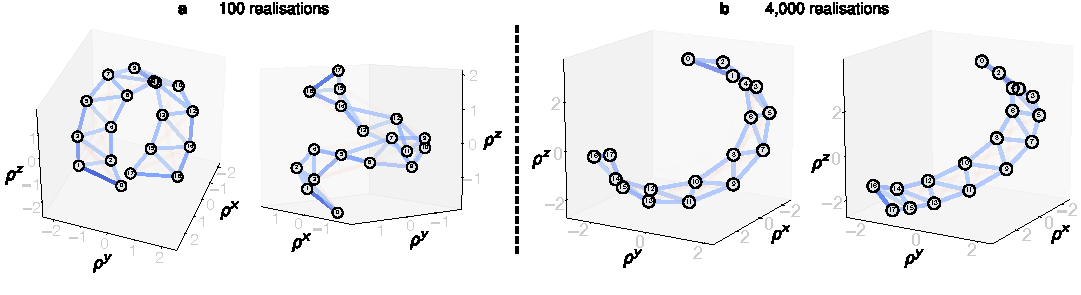
\includegraphics[width=\textwidth]{Figures/Supplement1.pdf}
    \caption{\textbf{Reconstructed Geometry for the anti-ferromagnetic ladder:} \textbf{a} shows two examples of the simulation results with 100 realizations. \textbf{b} shows two examples with 4,000 realizations each.}
    \label{Fig:SuppAFM_Ladder}
\end{figure}
\subsubsection{Treelike Correlations}
Using the TWA simulation, we also study the time evolution of the system with non-Archimedean geometry, i.e. the model of Eq.~\eqref{eq:tree_couplings} with $s = 1$.  We compare the simulation to the experimental data shown in Fig.~\ref{fig:trees}b for a fixed evolution time of two Bloch periods. The time evolution of the simulated data is depicted in Fig.~\ref{Fig:Supp_Tree}. After rearranging the sites according to the Monna map, we find that the simulated spin-spin correlations begin to exhibit a block structure after 2 Bloch periods of evolution time, much as in the experiment. The simulation additionally shows that the complete block structure expected for a treelike geometry only becomes fully visible for longer evolution times. In particular, after two Bloch periods the $8\times 8$ block corresponding to correlations between sites with a physical distance $\abs{i-j}=1$ is not yet clearly visible, which is consistent with our experimental findings.
\begin{figure}
    \centering
    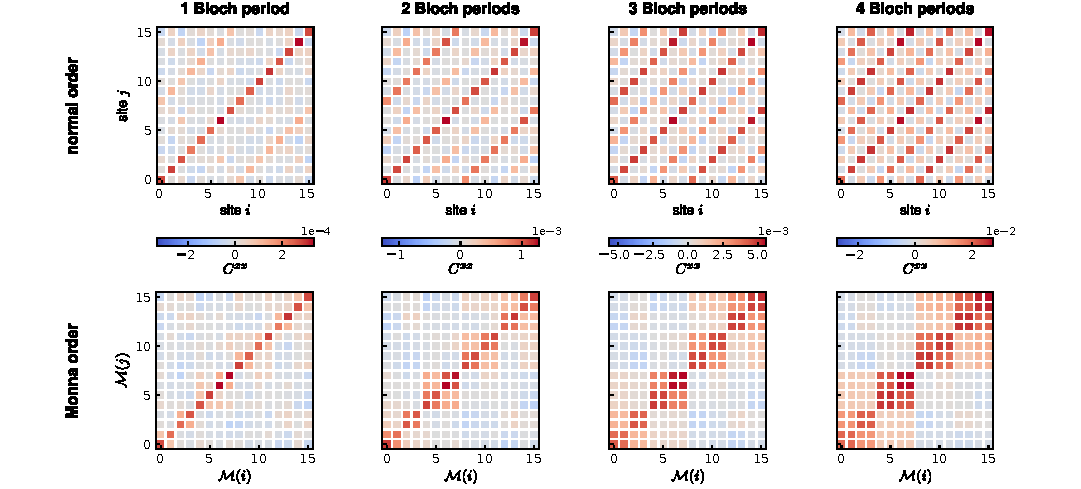
\includegraphics[width=\textwidth]{Figures/Supplement2.pdf}
    \caption{\textbf{TWA simulation of treelike correlation spreading.} The upper row depicts the spreading of correlations for the case of $s =1 $ as a function of time. The lower half shows the same data after rearranging the sites according to the Monna map. In the Monna-mapped case, one sees that the square structure builds up over time, which is a hallmark of the treelike geometry.}
    \label{Fig:Supp_Tree}
\end{figure}

\subsubsection{Bipartite Correlations}
Finally, we use the TWA simulation to study the effect of experimental noise on the measurement of bipartite correlations shown in Fig~\ref{fig:trees}\,c. The results are summarized in Fig.~\ref{Fig:Supp_Bipartite}. We compare the experimental and simulation results at $T=2$ and $T=3$ Bloch periods of evolution time. If we consider no experimental imperfection in the simulation, the extracted bipartite correlations in the simulation show qualitative agreement with the experiment as a function of the parameter $s$. However, especially for low correlations in the simulation, the experimentally extracted correlations are significantly larger.

For a more accurate simulation of the experimental situation, we include two known experimental imperfections into the TWA simulation. Firstly, we include magnetic field fluctuations as explained before. In addition, we account for classical correlations between neighbouring ensembles due to the finite resolution of the fluorescence imaging. We expect that the magnetic field fluctuations lead to a reduction of correlations, while the imaging resolution increases the correlations especially in the Monna mapped case. Including these two effects in the simulation improves the agreement with the experimental data, especially for the Monna-mapped ordering.

In the experiment, there are still excess correlations in the physically ordered case for $s<0$. These may be due to decoherence effects, together with a slight difference in detection efficiency between the magnetic substates $\pm1$. Together these effects could explain the overall increase of correlation which we observe especially for the physical ordering of sites.
\begin{figure}
    \centering
    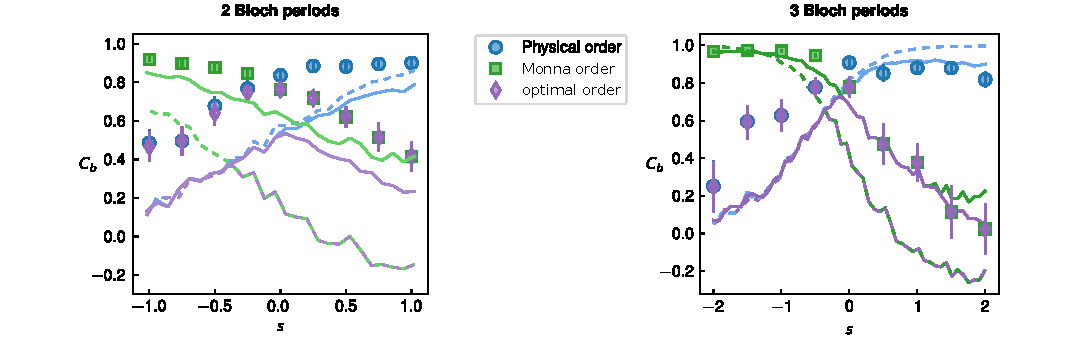
\includegraphics[width=\textwidth]{Figures/Supplement3.pdf}
    \caption{\textbf{Bipartite Correlations:} Comparison between the experimental data and simulation results for the bipartite correlations as functions of the parameter $s$. The plot markers show experimental data, while the solid and dashed lines are the corresponding simulation results with and without additional fluctuations, respectively. Here, we compare the simulation and the experimental data at $T=2$ (left) and $T=3$ (right) Bloch periods. In the simulation we have assumed that about 9\% (left plot) and 12\% (right plot) of the fluorescence signal at each site contributes crosstalk to the fluorescence signal at each neighboring site.}
    \label{Fig:Supp_Bipartite}
\end{figure}

\normalem
\putbib[programmable]
\end{bibunit}
\end{document}